\documentclass[a4paper,14pt]{extarticle} 
\usepackage[a4paper,top=1.5cm, bottom=1.5cm, left=2cm, right=1cm]{geometry}
%\usepackage[T2A]{fontenc}
%\usepackage[english, russian]{babel}
\usepackage{graphicx}
\graphicspath{{./pics/}}
\DeclareGraphicsExtensions{.pdf,.png,}

\usepackage{fontspec}
\setmainfont{Times New Roman}
\setsansfont{FreeSans}
\setmonofont{FreeMono}
\renewcommand{\baselinestretch}{1.5}
\usepackage{polyglossia}
\setdefaultlanguage{russian}
\setotherlanguages{english,russian}
\usepackage{setspace}
\usepackage[many]{tcolorbox}

\begin{document}
    \begin{center}
        \thispagestyle{empty}
        \begin{singlespace}
        ФЕДЕРАЛЬНОЕ АГЕНТСТВО СВЯЗИ

        ФЕДЕРАЛЬНОЕ ГОСУДАРСТВЕННОЕ БЮДЖЕТНОЕ ОБРАЗОВАТЕЛЬНОЕ

        УЧРЕЖДЕНИЕ ВЫСШЕГО ОБРАЗОВАНИЯ

        «САНКТ-ПЕТЕРБУРГСКИЙ ГОСУДАРСТВЕННЫЙ УНИВЕРСИТЕТ ТЕЛЕКОММУНИКАЦИЙ ИМ. ПРОФ. М.А. БОНЧ-БРУЕВИЧА»

        (СПбГУТ)
        \end{singlespace}
        \vspace{-1ex}
        \rule{\textwidth}{0.4pt}
        \vspace{-5ex}

        \vspace{100px}
        \textbf{Лабораторная работа №3}\\
        Исследование свойств модели резисторного касакада с общим колектором в частотной и временной областях на ПК

    \vspace{100px}
    \end{center}
    \vspace{4ex}
    \begin{flushright}
    \parbox{12 cm}{
    \begin{flushleft}
        Выполнила бригада:\\
        Группа ИКТЗ-83\\
        \underline{Громов А.А., Миколаени М.С., Мазеин Д.С.} \hfill \rule[-0.85ex]{0.09\textwidth}{0.6pt}\\
        \vspace{-1ex}
        \footnotesize \textit{ (Ф.И.О., № группы) \hfill (подпись)} \normalsize


    \end{flushleft}
    }
    \end{flushright}
    \begin{center}
        \vfill
        Санкт-Петербург

        2020

    \end{center}
    \newpage

    \textbf{Цель работы:} Изучить свойства усилительного каскада с общим коллектором (ОК) в режиме малого сигнала. Выполнить анализ в частотной и временной областях. Исследовать свойства каскада при изменении сопротивлений источника сигнала, нагрузки и элементов схемы. Определить входное и выходное сопротивления каскада.

    \textbf{Пункт 1:}
    \begin{center}
        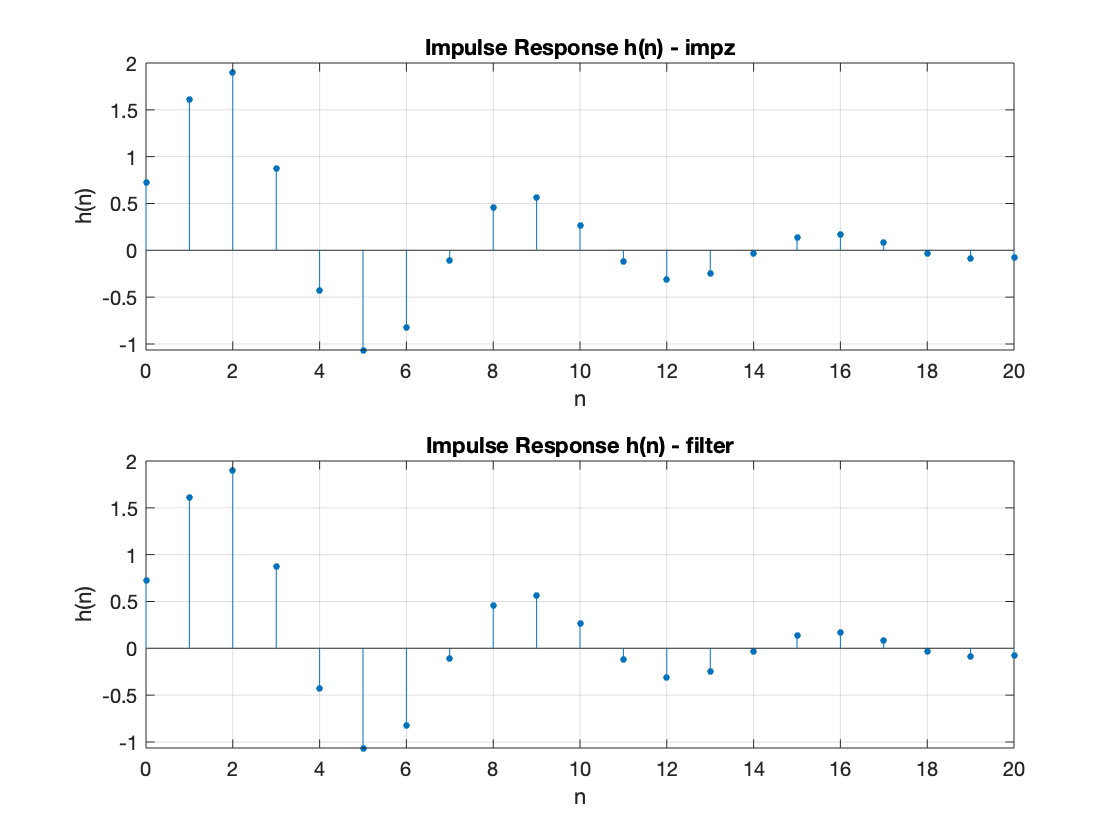
\includegraphics{1}
    \end{center}

\end{document}